\typeout{NT FILE IMPLEM.tex}%
\chapter{Implementation}
\label{cha:implementation}

\section{Workflow}
\label{sec:workflow}
Fig.~\ref{fig:uav-main-Implem-Workflow} illustrates the overall implementation
workflow: the \gls{uspfs} solution comprises the \textbf{Guests}, \textbf{Firmware},
and \textbf{Deployment} sections, and the \gls{sspfs} solution also includes the
\textbf{Hypervisor} section. On the left we can see the four major
implementation's steps: \textbf{Build guests},
\textbf{Build Hypervisor and VMs} (\gls{sspfs} only), \textbf{Build Firmware},
and \textbf{Deployment}. The term ``guest'' is used loosely here, meaning an
actual guest that executes atop of the Bao hypervisor in the \gls{sspfs} case,
or a binary that runs natively on the \gls{uavic} platform (\gls{uspfs}).

\begin{figure}[!hbt]
  \centering
  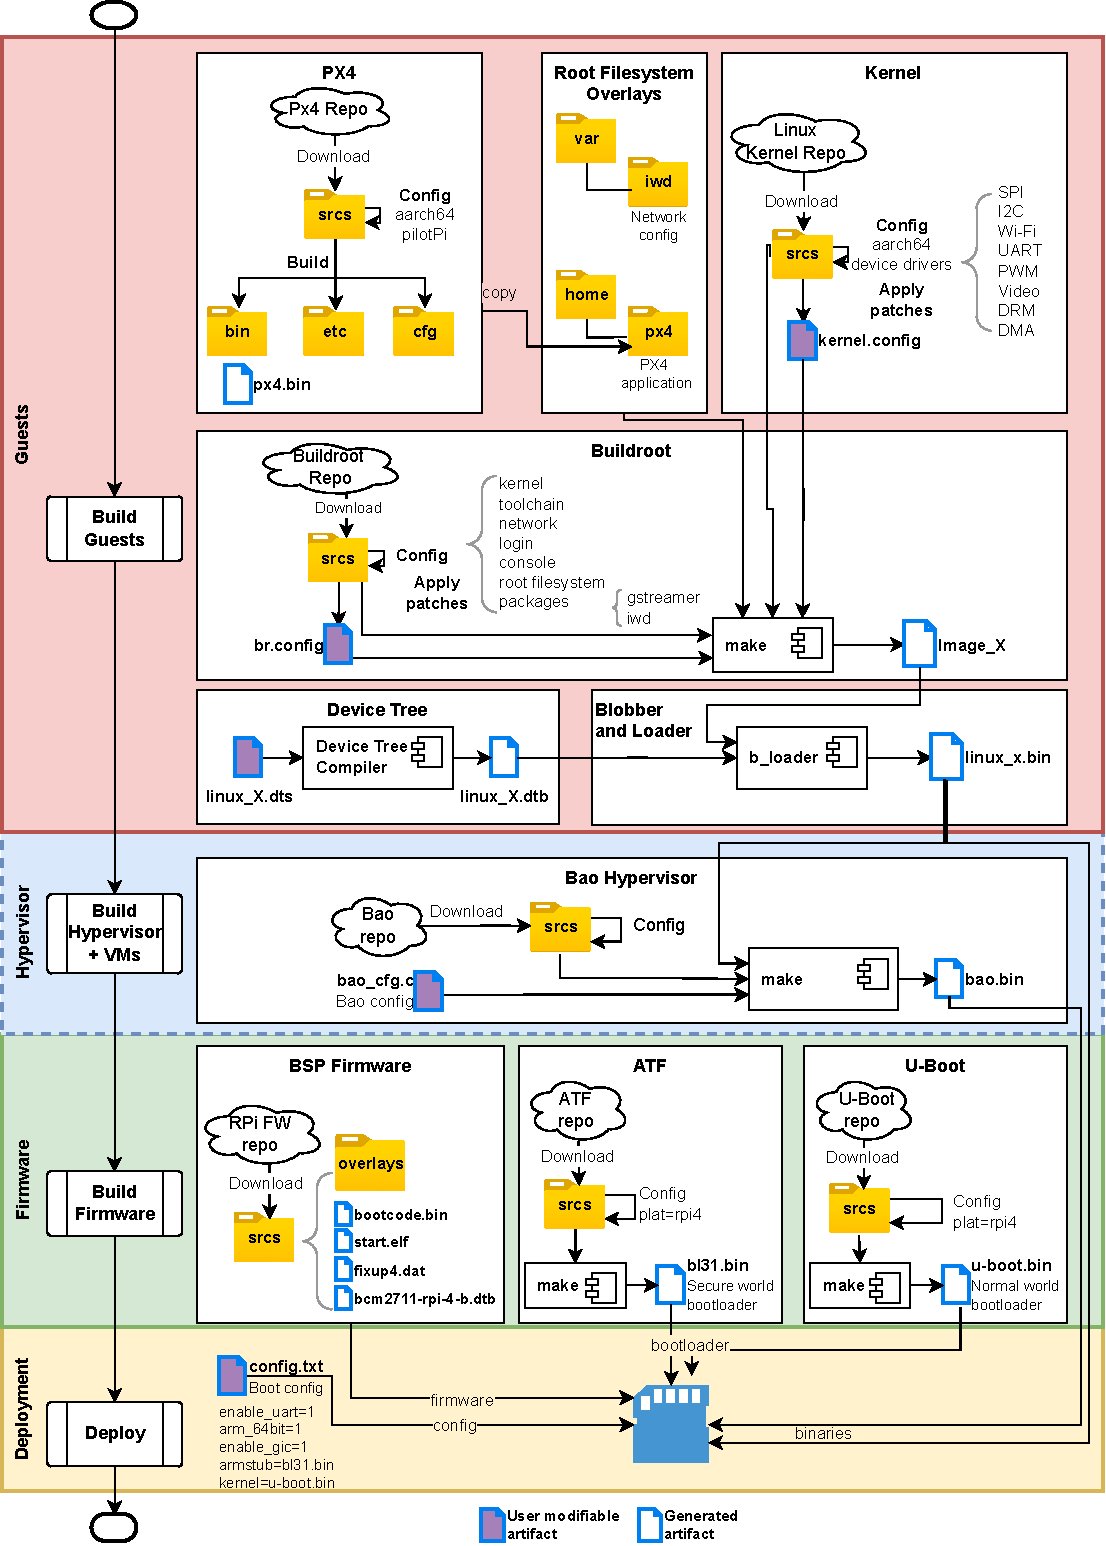
\includegraphics[width=1.0\textwidth]{./img/pdf/uav-main-Implem-Workflow} 
  \caption{Implementation workflow}%
  \label{fig:uav-main-Implem-Workflow}
\end{figure}

The first step is to build the guests. Only one ``guest'' can run natively at a
time in the \gls{uspfs} scenario, with
PX4 and video surveillance features encompassed in a single binary. On the other
hand, PX4 and video surveillance guests execute simultaneously and in isolation
in the \gls{sspfs} scenario. Thus, we start by building the PX4 application to
run on the \texttt{PilotPi} board with the \texttt{aarch64} architecture,
yielding a set of binaries and configuration files that can be deployed to the
\gls{uavic} platform. Then, we copy these files to a special directory --- the
Root Filesystem Overlays --- alongside with the network configuration to be
deployed by the selected embedded Linux build system (Buildroot) when compiling
the guest binary.
Next we configure the Linux kernel to add support for the required device
drivers, such as \gls{spi}, \gls{i2c}, Wi-Fi, video, among others. We then
configure the embedded system to include the preconfigured kernel and to deploy
the PX4 application to the target, alongside with the network, login, console
and packages (e.g., \texttt{gstreamer} for video and \texttt{iwd} for wireless
network setup). Buildroot compiles a Linux image \texttt{Image\_X}, where
\texttt{X} is the guest's number. Next, we configure the device tree source \texttt{linux\_X.dts} to
match the available hardware for each guest and compile it to generate a \gls{dtb} \texttt{linux\_X.dtb}. The \gls{dtb} is then wrapped together
with the Linux's guest image \texttt{Image\_X} by the \texttt{b\_loader}
component, yielding an executable that can be deployed to the \gls{uavic}
platform with minimal dependencies and matching the required hardware. In the
\gls{uspfs} case we have an unique binary to deploy; in the \gls{sspfs} case,
however, we need to repeat the process for each guest to comply with the
requirements, yielding two binaries which will later on be merged by the Bao
hypervisor when generating the target's executable.

Secondly, and only for the \gls{sspfs} case, we create a configuration for each
\gls{vm} describing the guest's available resources --- such as memory, number
of \glspl{cpu}, and the devices --- the entry point, and the interrupt
management. Each configuration file is matched to the respective guest's binary
to setup each guest in the Bao hypervisor and then merged to generate a unique
blob (\texttt{bao.bin}) containing the two guests atop of the hypervisor.

Next, we build the platform's firmware. We download the \gls{bsp} firmware for
the Raspberry Pi 4, containing the board's firmware, the first stage bootloader
and the device tree blob to boot the board. We configure and build the
\gls{atf} (\texttt{bl31.bin}), required by the Bao hypervisor. Then, we
configure and build the normal world bootloader (\texttt{u-boot.bin}), which
will be used to load the target binary --- \texttt{linux\_x.bin} in the
\gls{uspfs} case or \texttt{bao.bin} in the \gls{sspfs} case.

Lastly, we deploy the boot artifacts to the \gls{sd} card, containing the
Raspberry Pi 4 firmware, the secondary bootloaders, the target binary
(\texttt{linux\_x.bin} or \texttt{bao.bin}) and a configuration file
(\texttt{config.txt}). The configuration file sets up the boot process, enabling
the \gls{uart} and \gls{gic} subsystems, and pointing to the secondary
bootloaders which will be invoked after the initial board boot up is completed.


For further clarification of the deployment stage, it is important to analyze
the \gls{uavic} boot flow, depicted in Fig.~\ref{fig:uav-main-rpi4-boot}. The
first stage bootloader (\texttt{bootcode.bin}) initializes the hardware, loads
the firmware from the \gls{sd} card and reads the \texttt{config.txt} file to
parse the boot parameters.

\begin{figure}[!hbt]
  \centering
  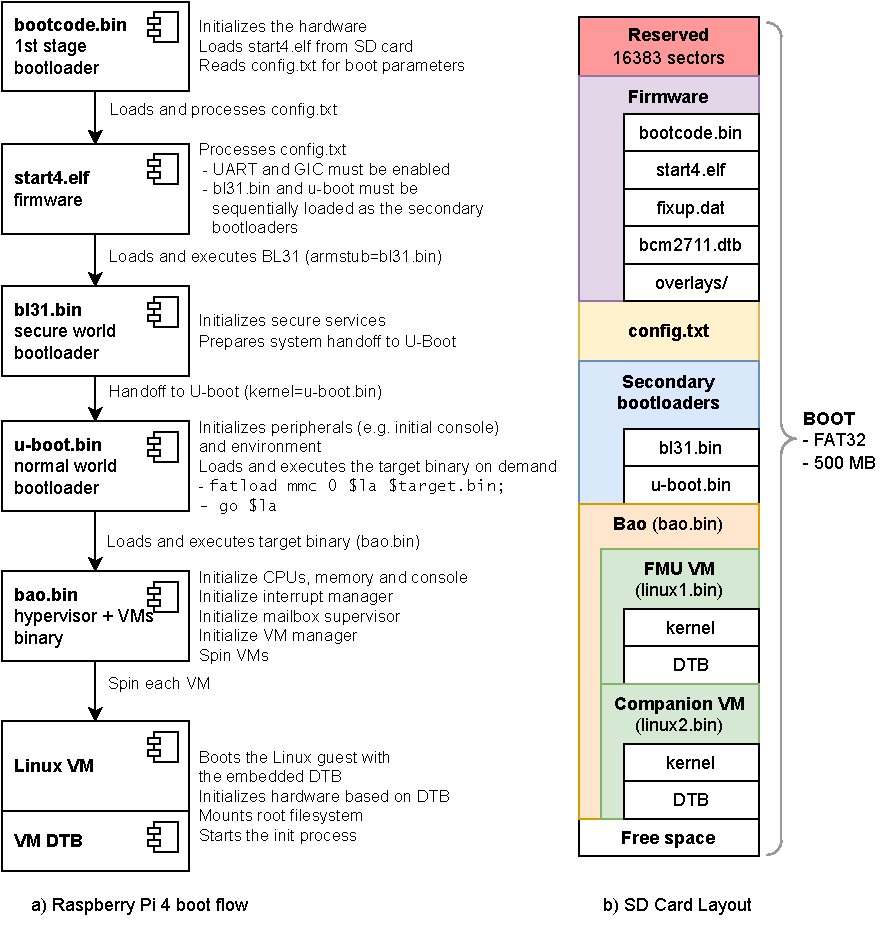
\includegraphics[width=0.9\textwidth]{./img/pdf/uav-main-rpi4-boot} 
  \caption{UAVIC boot: a) platform boot flow; b) SD card layout}%
  \label{fig:uav-main-rpi4-boot}
\end{figure}

The firwmare (\texttt{start4.elf}) processes config.txt, which in this case,
means it must enable \gls{uart} and \gls{gic} and that the secondary bootloaders
--- \texttt{bl31.bin} and \texttt{u-boot.bin} ---
must be sequentially loaded. 
%
It then loads and executes \texttt{bl31.bin} which initializes the secure
services and prepares system handoff to the normal world bootloader
\texttt{u-boot.bin}.
%
Next, control is handed to \texttt{u-boot.bin}, which initializes the peripherals
(e.g. initial console) based on the firmware's \gls{dtb} and the
environment. \texttt{u-boot.bin} allows to load and execute the target binary on
demand, whether through boot parameters stored in a U-Boot script or directly in the console.

The target binary is then executed: \texttt{linux\_x.bin} for the \gls{uspfs}
case or \texttt{bao.bin} for the \gls{sspfs} case. We will focus on the latter,
which is a superset of the former. The Bao hypervisor initializes the
\glspl{cpu}, memory and system console, the interrupt manager, the mailbox
supervisor, and, lastly, the \gls{vm} manager. After completing the
initialization it spins each \gls{vm} which boots the Linux guest with the
embedded \gls{dtb}, initializes the hardware based on the guest's configuration
file and the \gls{dtb}, mounts the root filesystem and starts the \texttt{init}
process. Each guest is now executing in isolation, supervised by the Bao hypervisor.

\section{USPFS}
\label{sec:uspfs-implem}

UAV Assembly

Build

\section{SSPFS}
\label{sec:sspfs-implem}

Bao Config

VM1

VM2

\subsection{Mailbox supervision}
\label{sec:mailbox-supervision}



\section{Summary}
\label{sec:summary-implem}



%%% Local Variables:
%%% mode: LaTeX
%%% TeX-master: "../template"
%%% End:
